\newcommand{\webscaleoutfig}{
    \begin{figure}[tb]
    \centering
    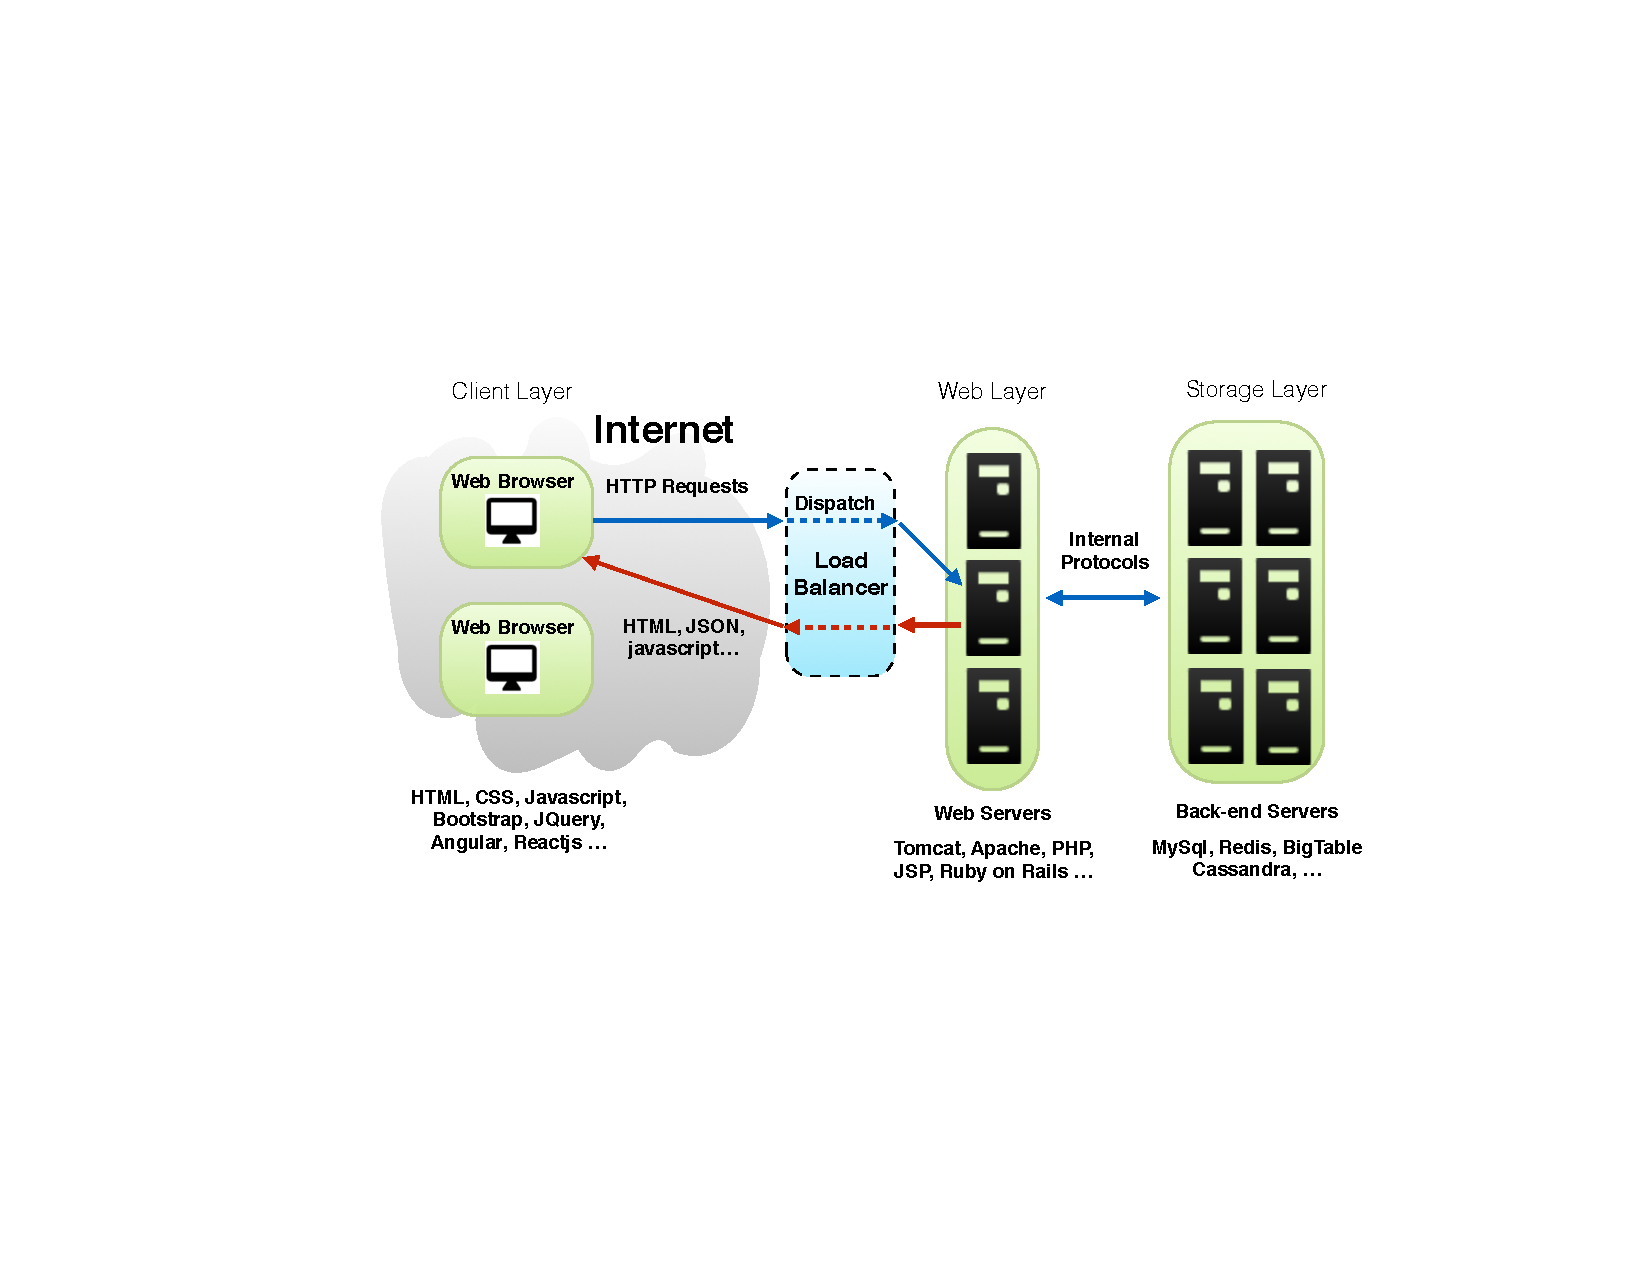
\includegraphics[width=\textwidth]{../figs/web_scale_out}
    \caption{Scalable web server architecture}
    \label{fig:webscaleout}
    \end{figure}
}

\newcommand{\architectureoverview}{
    \begin{figure*}[ht]
    \centering
    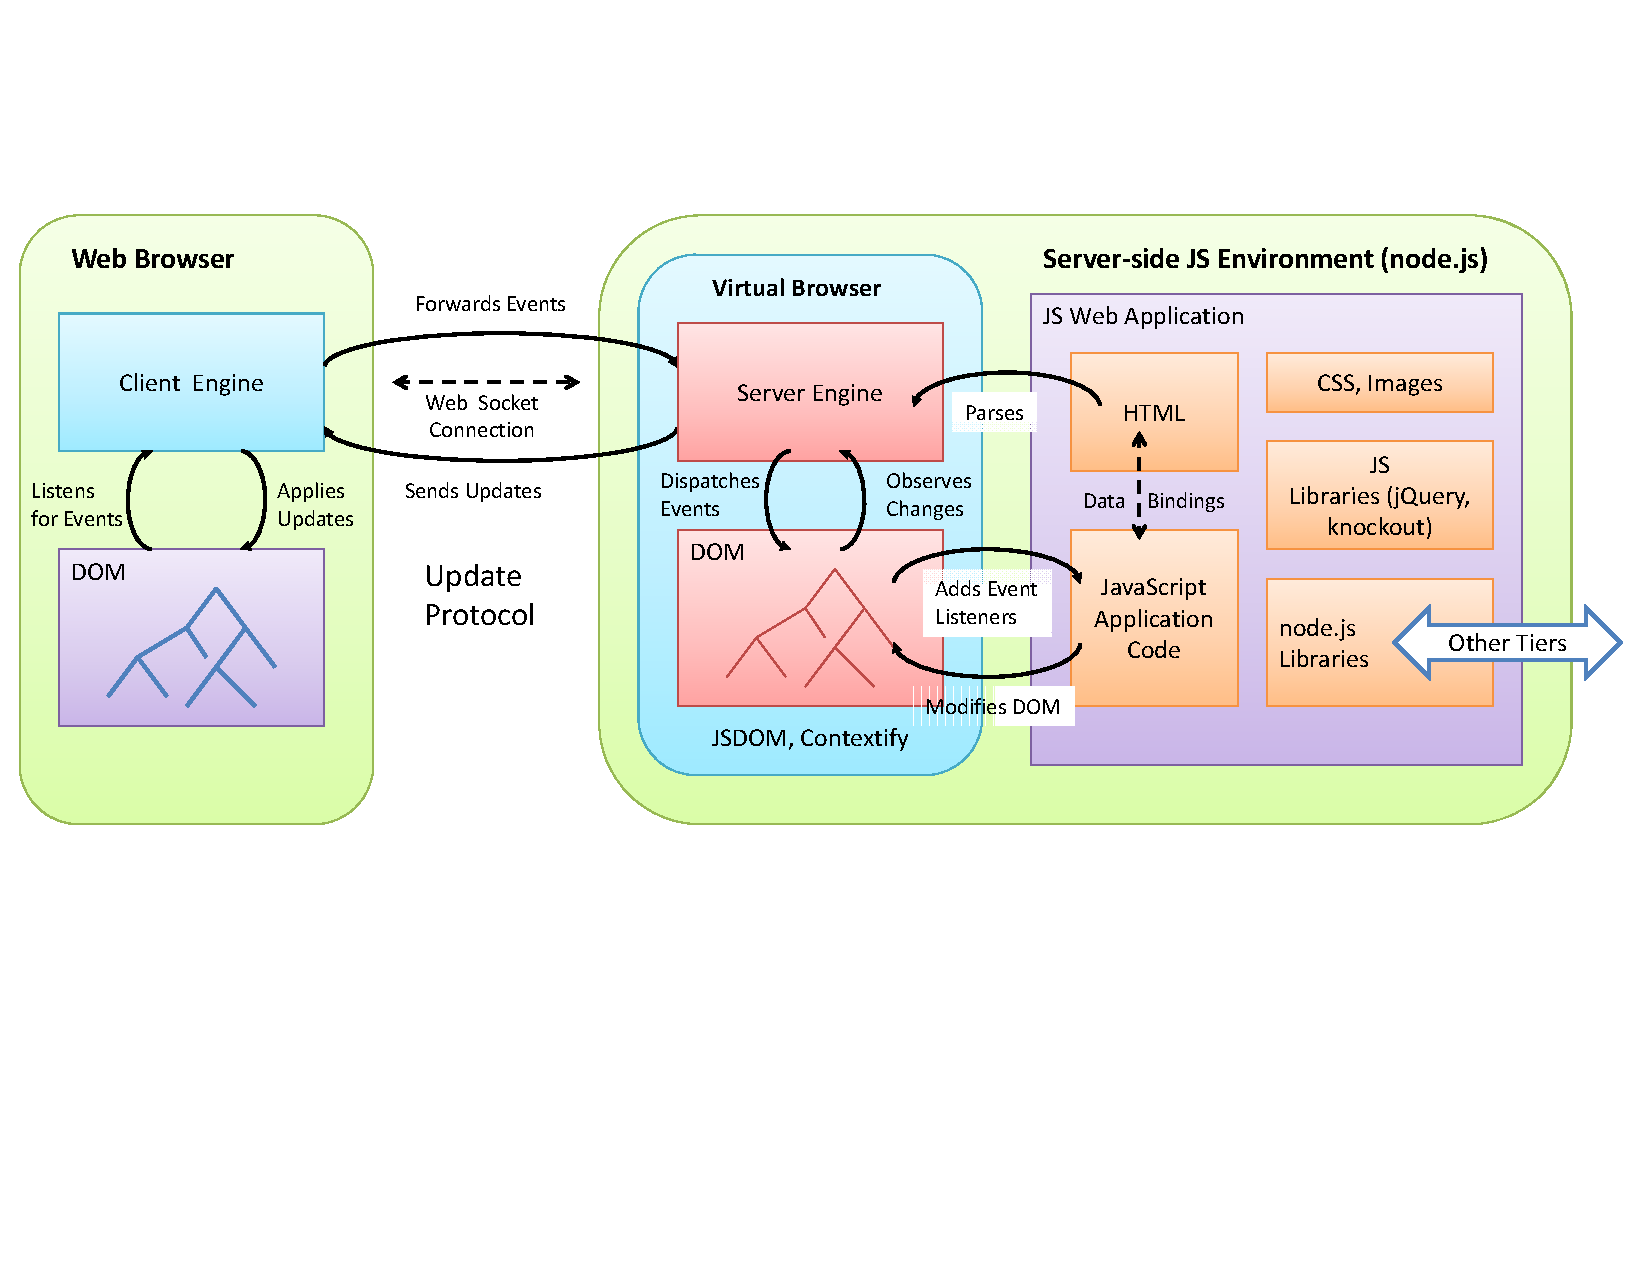
\includegraphics[width=\textwidth]{../figs/architecture_overview}
    \caption{Single Process \cb{} Architecture Overview}
    \label{fig:cb1arch}
    \end{figure*}
}

\newcommand{\newarchitectureoverview}{
    \begin{figure*}[ht]
    \centering
    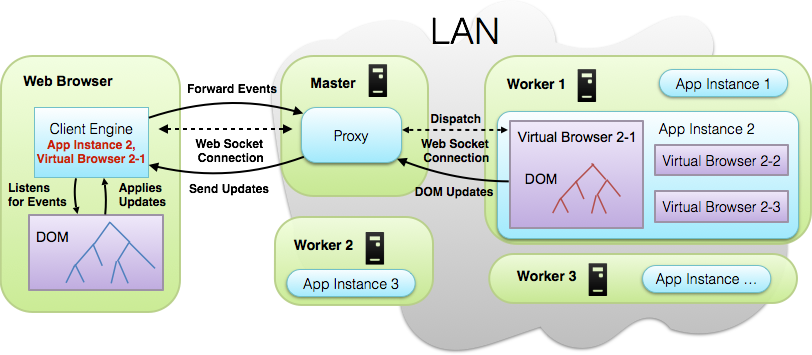
\includegraphics[width=\textwidth]{../figs/new_architecture_overview}
    \caption{Multiprocess Process \cb{} Architecture Overview}
    \label{fig:cb2arch}
    \end{figure*}
}


\newcommand{\appinstancefig}{
    \begin{figure}[ht]
    \centering
    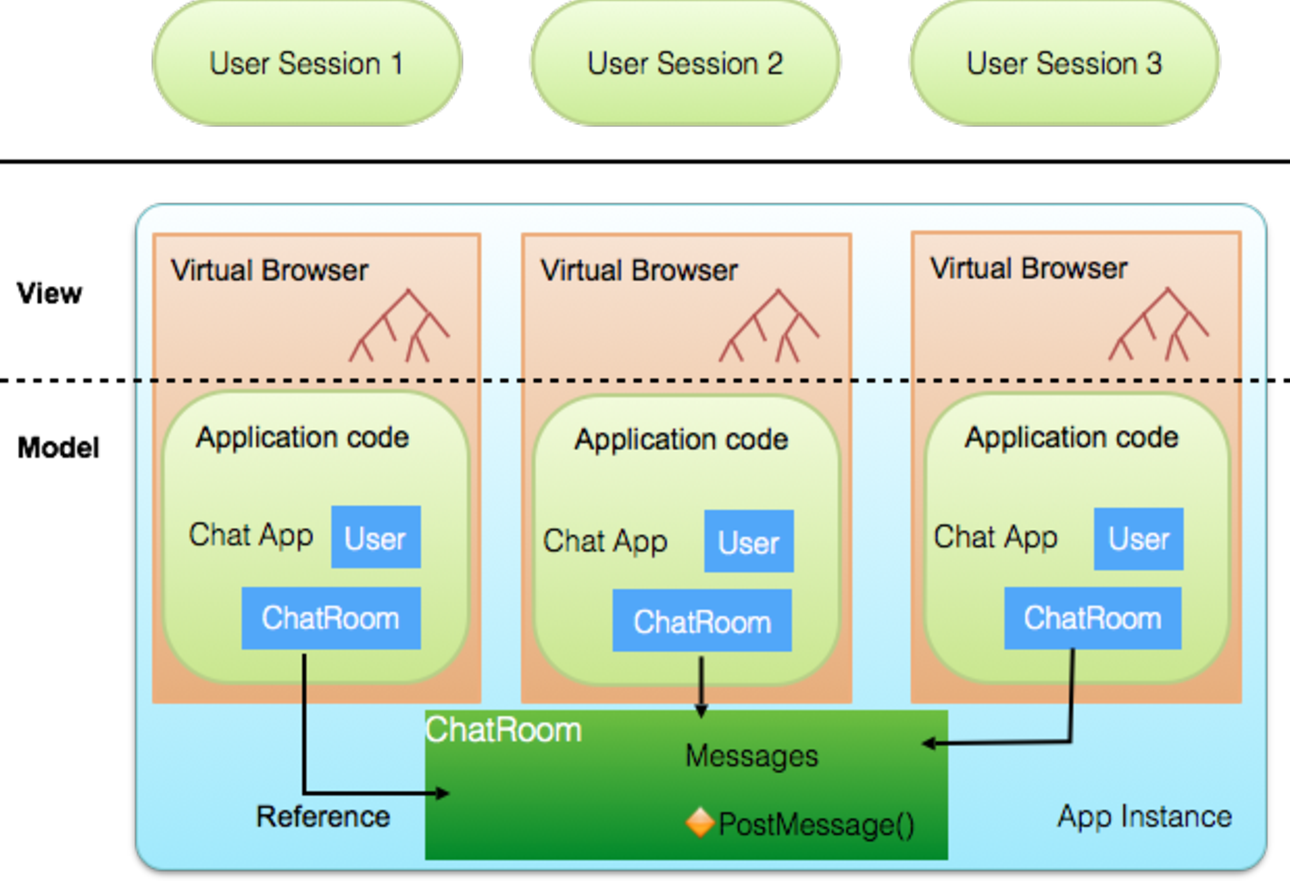
\includegraphics[width=0.8\textwidth]{../figs/appInstance}
    \caption{Application Instance}
    \label{fig:appinstance}
    \end{figure}
}


\newcommand{\appprojectfig}{
    \begin{figure}[ht]
    \centering
    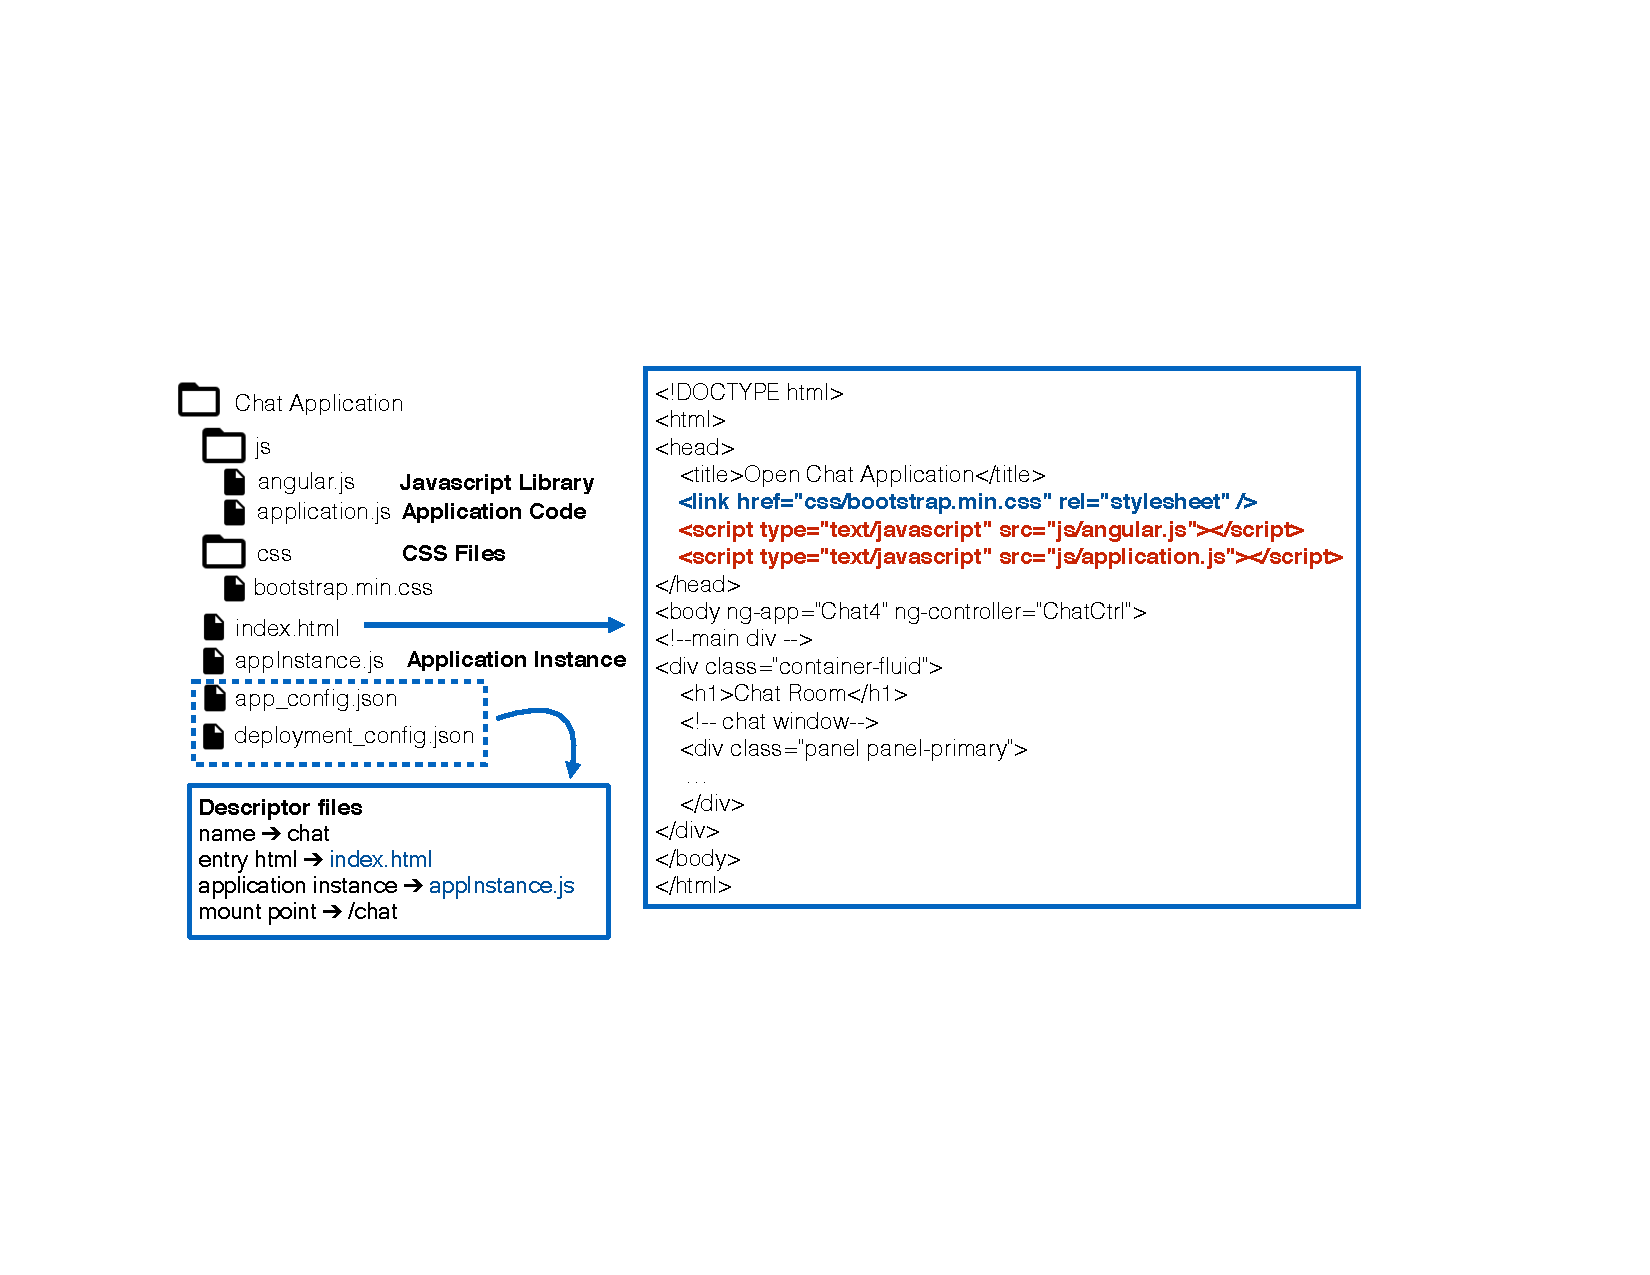
\includegraphics[width=\textwidth]{../figs/application_project}
    \caption{Folder structure of a \cb application}
    \label{fig:appproject}
    \end{figure}
}

\newcommand{\chatappfig}{
    \begin{figure}[ht]
    \centering
    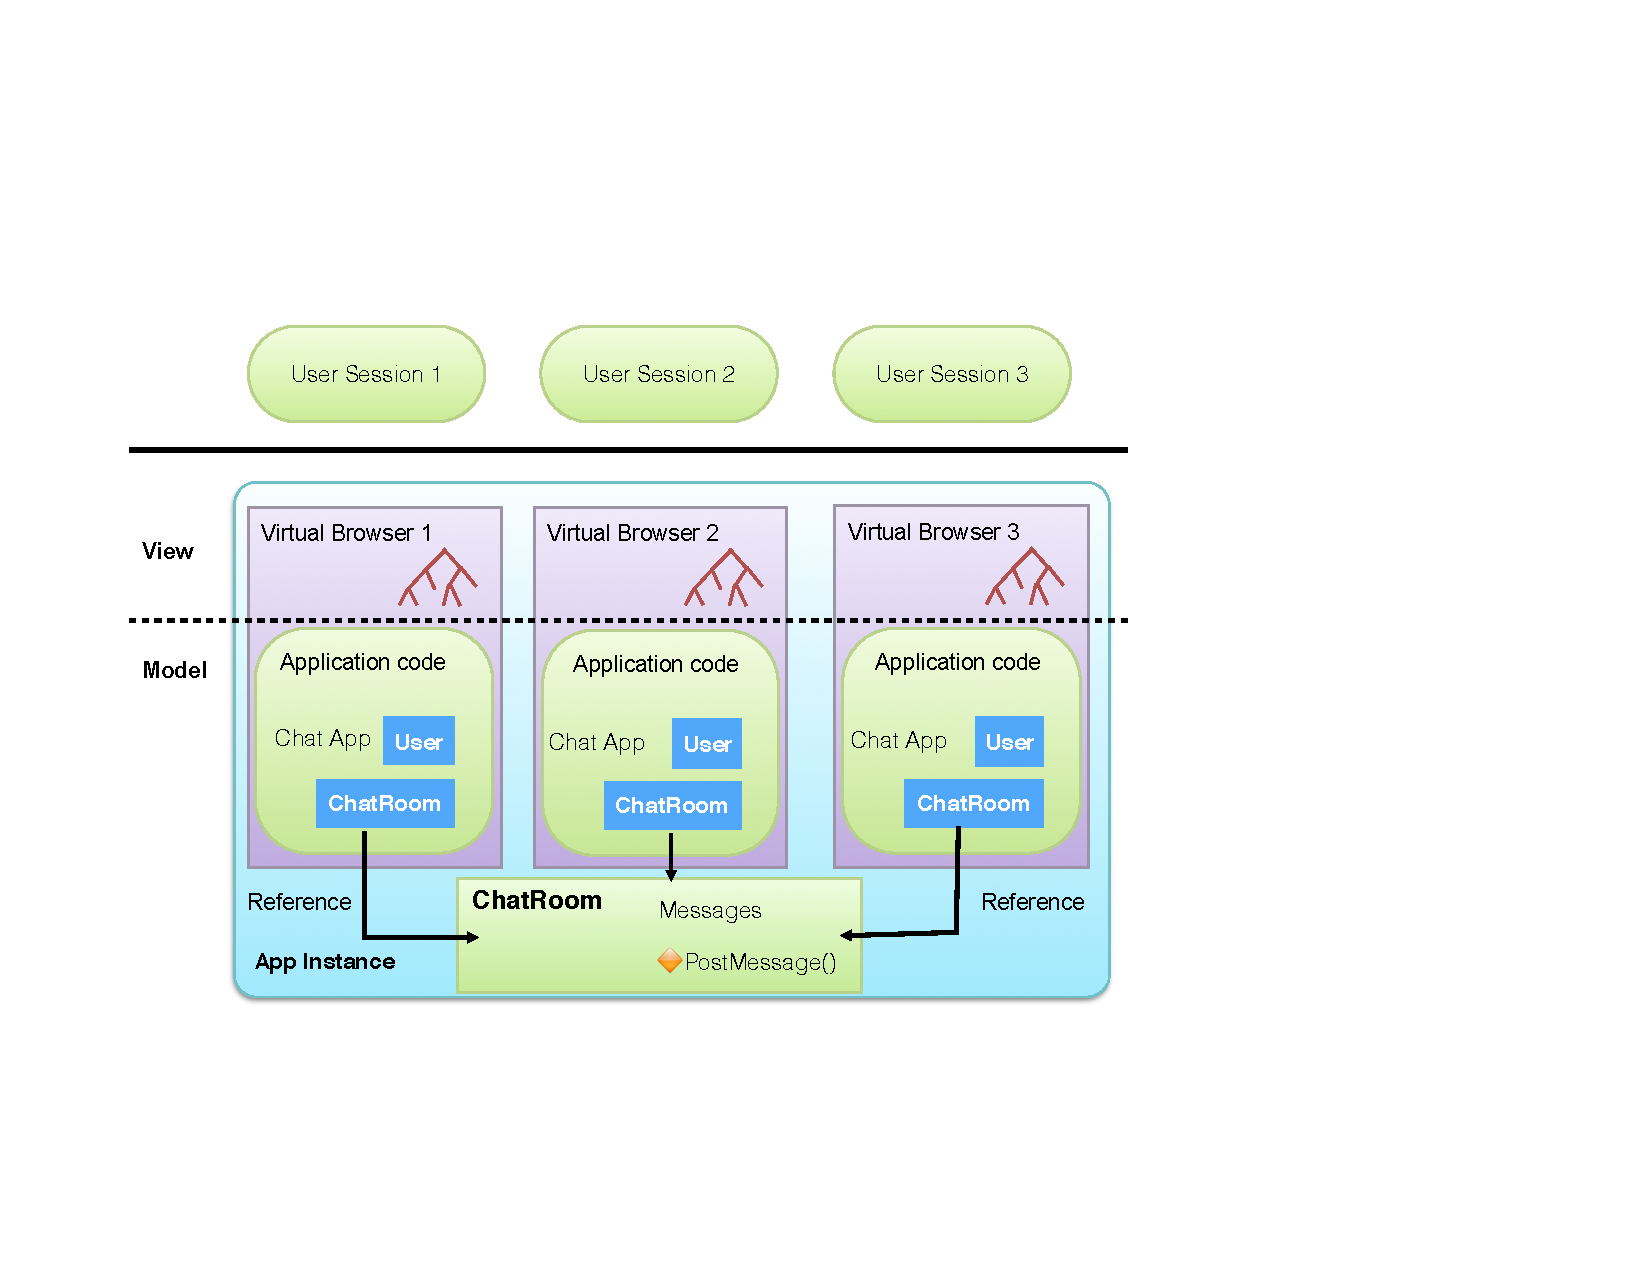
\includegraphics[width=0.8\textwidth]{../figs/chat_application}
    \caption[Sharing data among multiple virtual browser via application instance]
        {This figure shows how multiple virtual browsers can directly,
        and seamlessly share relevant application data, in this case chat messages,
        which then become part of the model that drives the presentation
        MVC framework.
    }
    \label{fig:chatapp}
    \end{figure}
}


\newcommand{\clickthroughput}{
    \begin{figure}[ht]
    \centering
    \includegraphics[width=\textwidth]{../gnuplot/click_throughput}
    \caption{Throughput of ``Back-to-back'' click application.}
    \label{fig:clickthroughput}
    \end{figure}
}


\newcommand{\clicklatency}{
    \begin{figure}[ht]
    \centering
    \includegraphics[width=\textwidth]{../gnuplot/click_latency}
    \caption{Latency of ``Back-to-back'' click application.}
    \label{fig:clicklatency}
    \end{figure}
}


\newcommand{\clickwaitthroughput}{
    \begin{figure}[ht]
    \centering
    \includegraphics[width=\textwidth]{../gnuplot/click_wait_throughput}
    \caption{Throughput of click application, after introducing artificial delay.}
    \label{fig:clickwaitthroughput}
    \end{figure}
}


\newcommand{\clickwaitlatency}{
    \begin{figure}[tb]
    \centering
    \includegraphics[width=\textwidth]{../gnuplot/click_wait_latency}
    \caption{Latency of click application, after introducing artificial delay.}
    \label{fig:clickwaitlatency}
    \end{figure}
}



\newcommand{\angularchatlatency}{
    \begin{figure}[tb]
    \centering
    \includegraphics[width=\textwidth]{../gnuplot/angularchat_latency}
    \caption{Latency of chat application with Angular.js.}
    \label{fig:angularchatlatency}
    \end{figure}
}


\newcommand{\jquerychatlatency}{
    \begin{figure}[tb]
    \centering
    \includegraphics[width=\textwidth]{../gnuplot/jquerychat_latency}
    \caption{Latency of chat application with JQuery.}
    \label{fig:jquerychatlatency}
    \end{figure}
}


\newcommand{\chatroomfig}{
    \begin{figure}[tb]
    \centering
    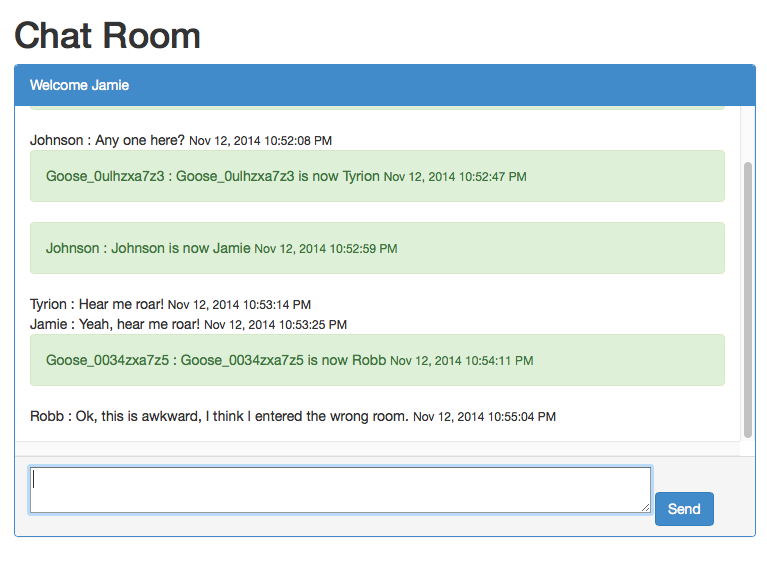
\includegraphics[width=\textwidth]{../figs/chatroom}
    \caption{Chat Room Application}
    \label{fig:chatroom}
    \end{figure}
}

\newcommand{\apphierarchyfig}{
    \begin{figure}[tb]
    \centering
    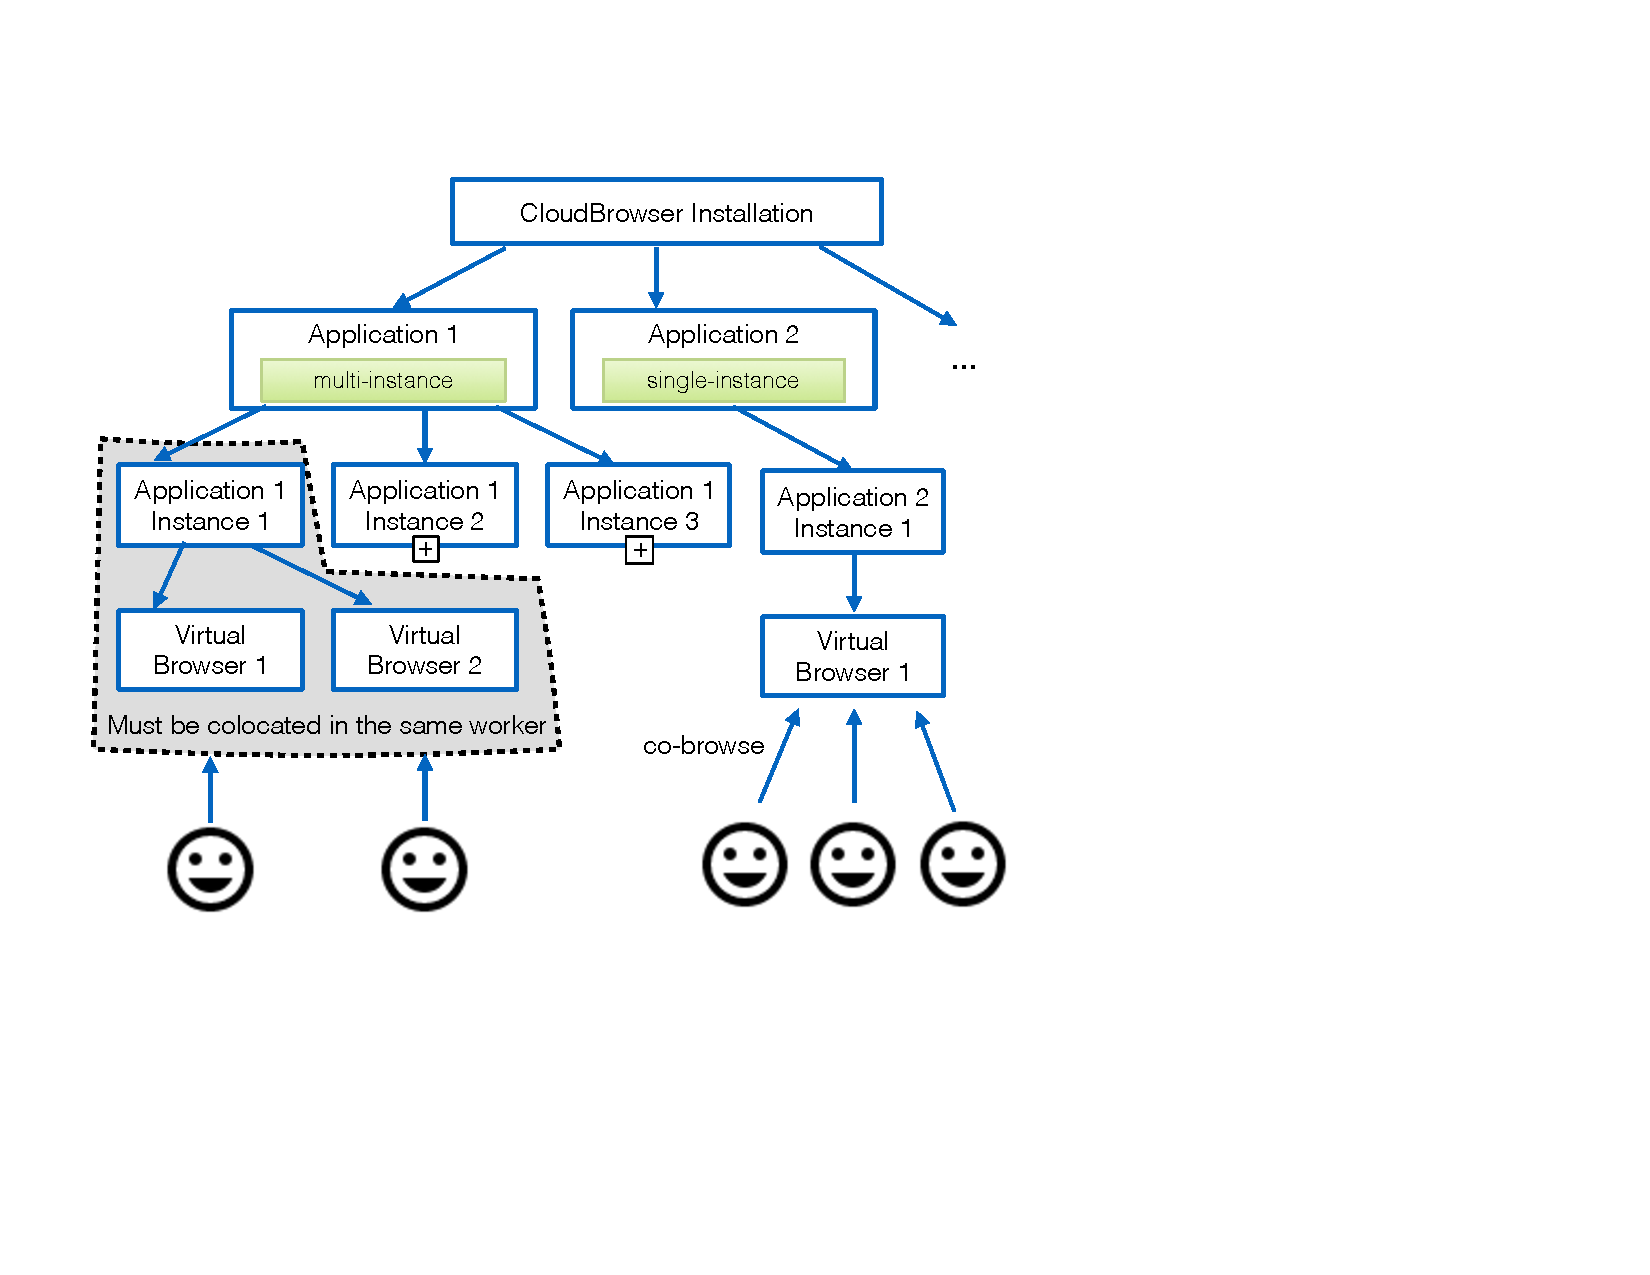
\includegraphics[width=0.8\textwidth]{../figs/application_hierarchy}
    \caption[Application deployment model]{Application deployment model: Hierarchy of applications, application instances, and virtual browsers.
    Note that a single virtual browser may be broadcast to multiple clients (cobrowsing).}
    \label{fig:appidhierarchy}
    \end{figure}
}

\newcommand{\memfig}{
\begin{figure*}[ht]
    \centering
    \includegraphics[width=\textwidth]{../gnuplot/resource_consumption}
    \caption[Resource Consumption of worker]{
    Resource Consumption of worker node running JQueryChat Application\\
X axis is time. Left Y axis corresponds to the red line of CPU usage.
Right Y axis corresponds to memory statistics.\\
After about 90s after the system boots up, the benchmark tool starts to simulate 
user workload.
When the benchmark tool sending requests, \emph{HeapUsed} fluctuates as the system creates new objects and garbage collector cleans dead objects.
When the \emph{HeapUsed} drops there is a steep surge of CPU usage, indicating garbage collector is working at that time.
    }
    \label{fig:mem}
\end{figure*}
}


\newcommand{\nodermifig}{
    \begin{figure}[ht]
    \centering
    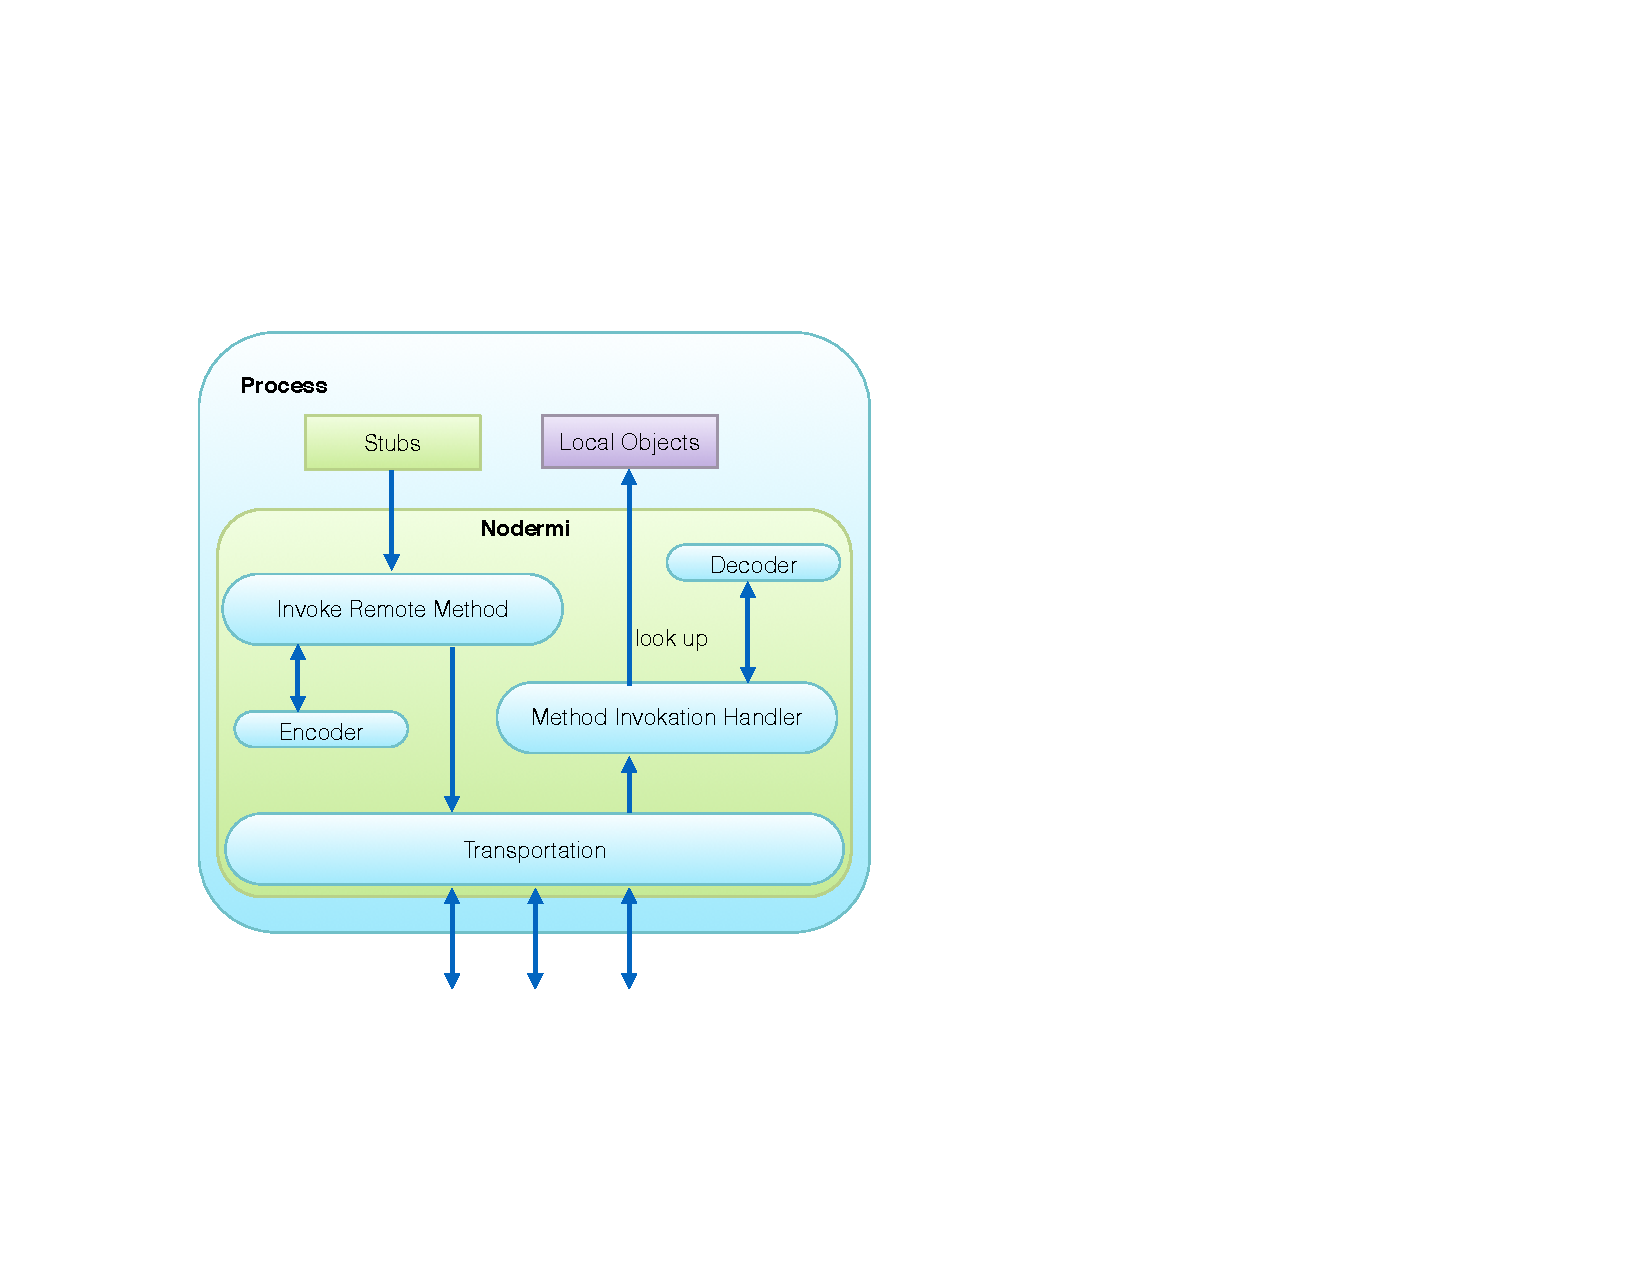
\includegraphics[width=\textwidth]{../figs/nodermi}
    \caption[Overall Design of nodermi]{Overall Design of nodermi}
    \label{fig:nodermi}
    \end{figure}
}

% deprecated
\newcommand{\nodermimethodinvokefig}{
    \begin{figure}[ht]
    \centering
    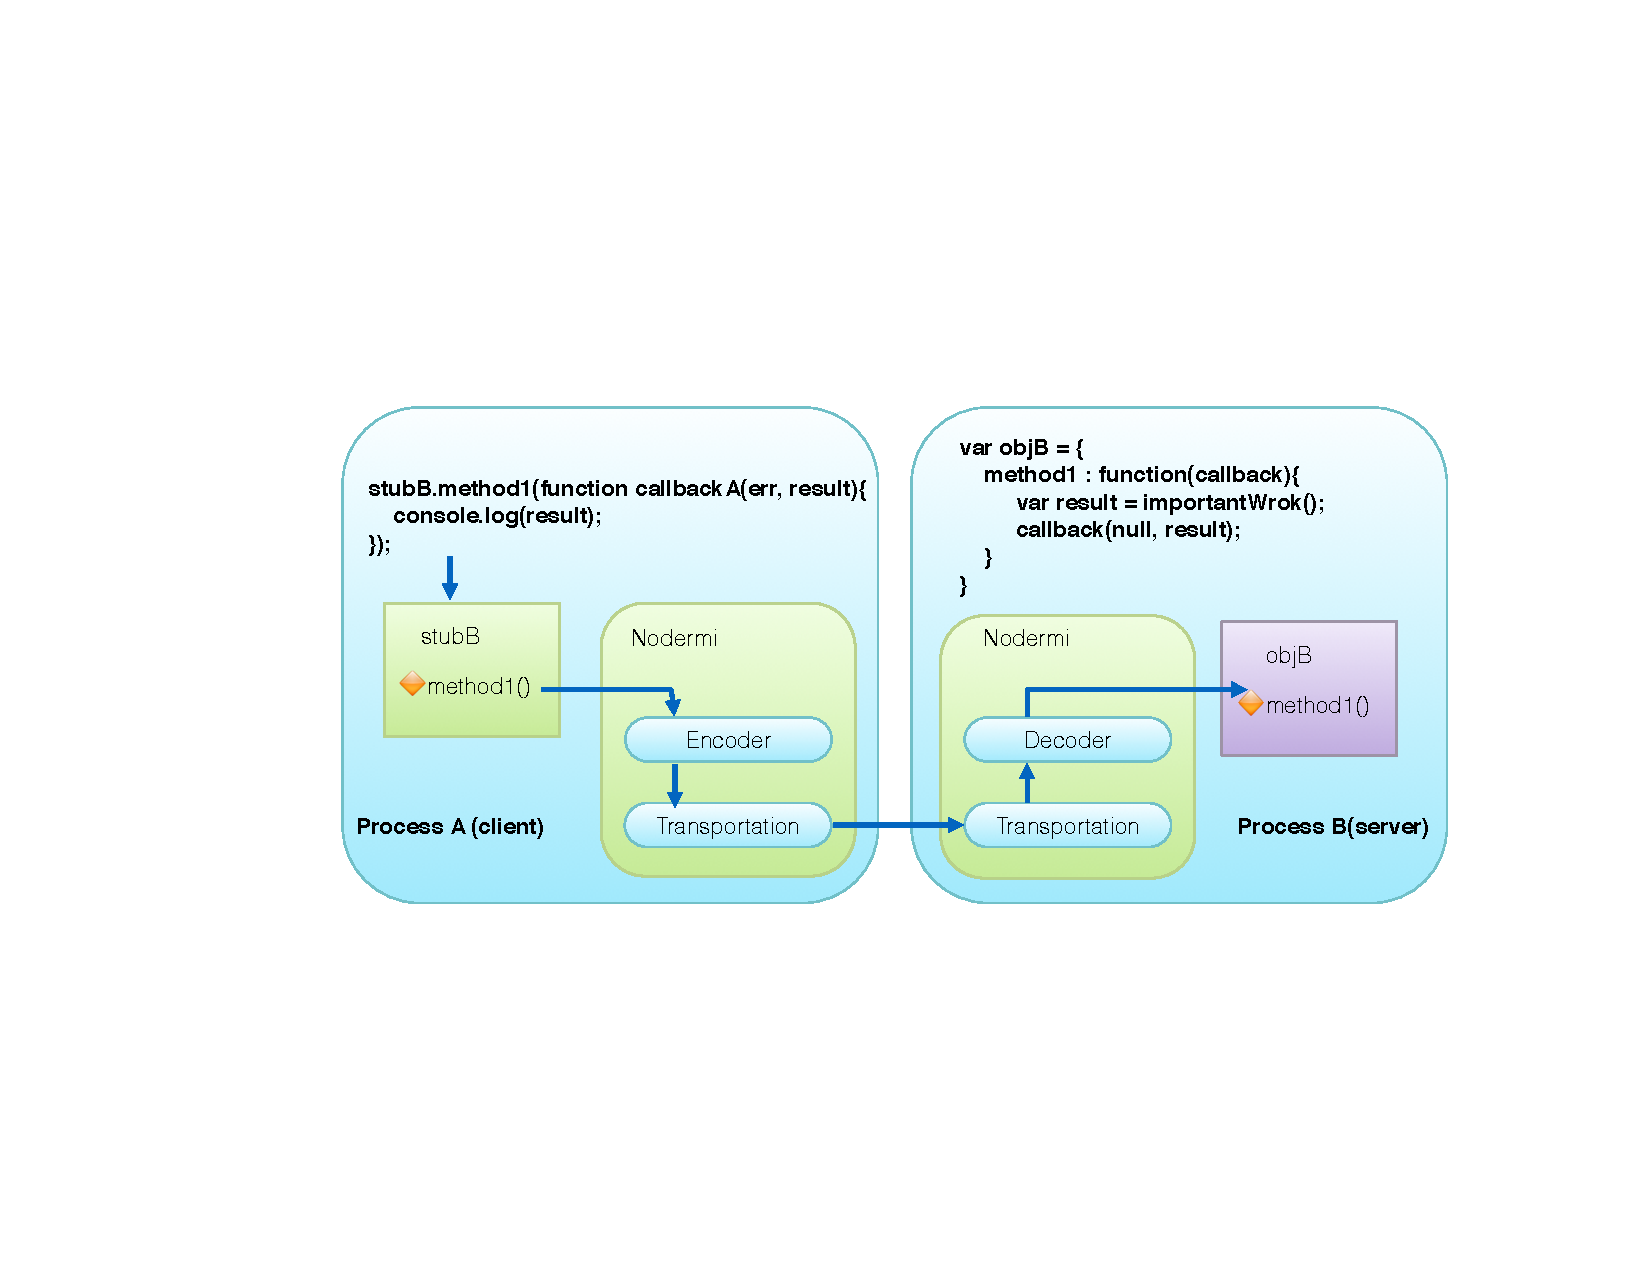
\includegraphics[width=0.8\textwidth]{../figs/nodermi_method_invoke}
    \caption[Remote method invocation via a stub object]{Process A invoke a method of a stub object}
    \label{fig:nodermimethodinvoke}
    \end{figure}
}

% deprecated
\newcommand{\nodermicallbackfig}{
    \begin{figure}[ht]
    \centering
    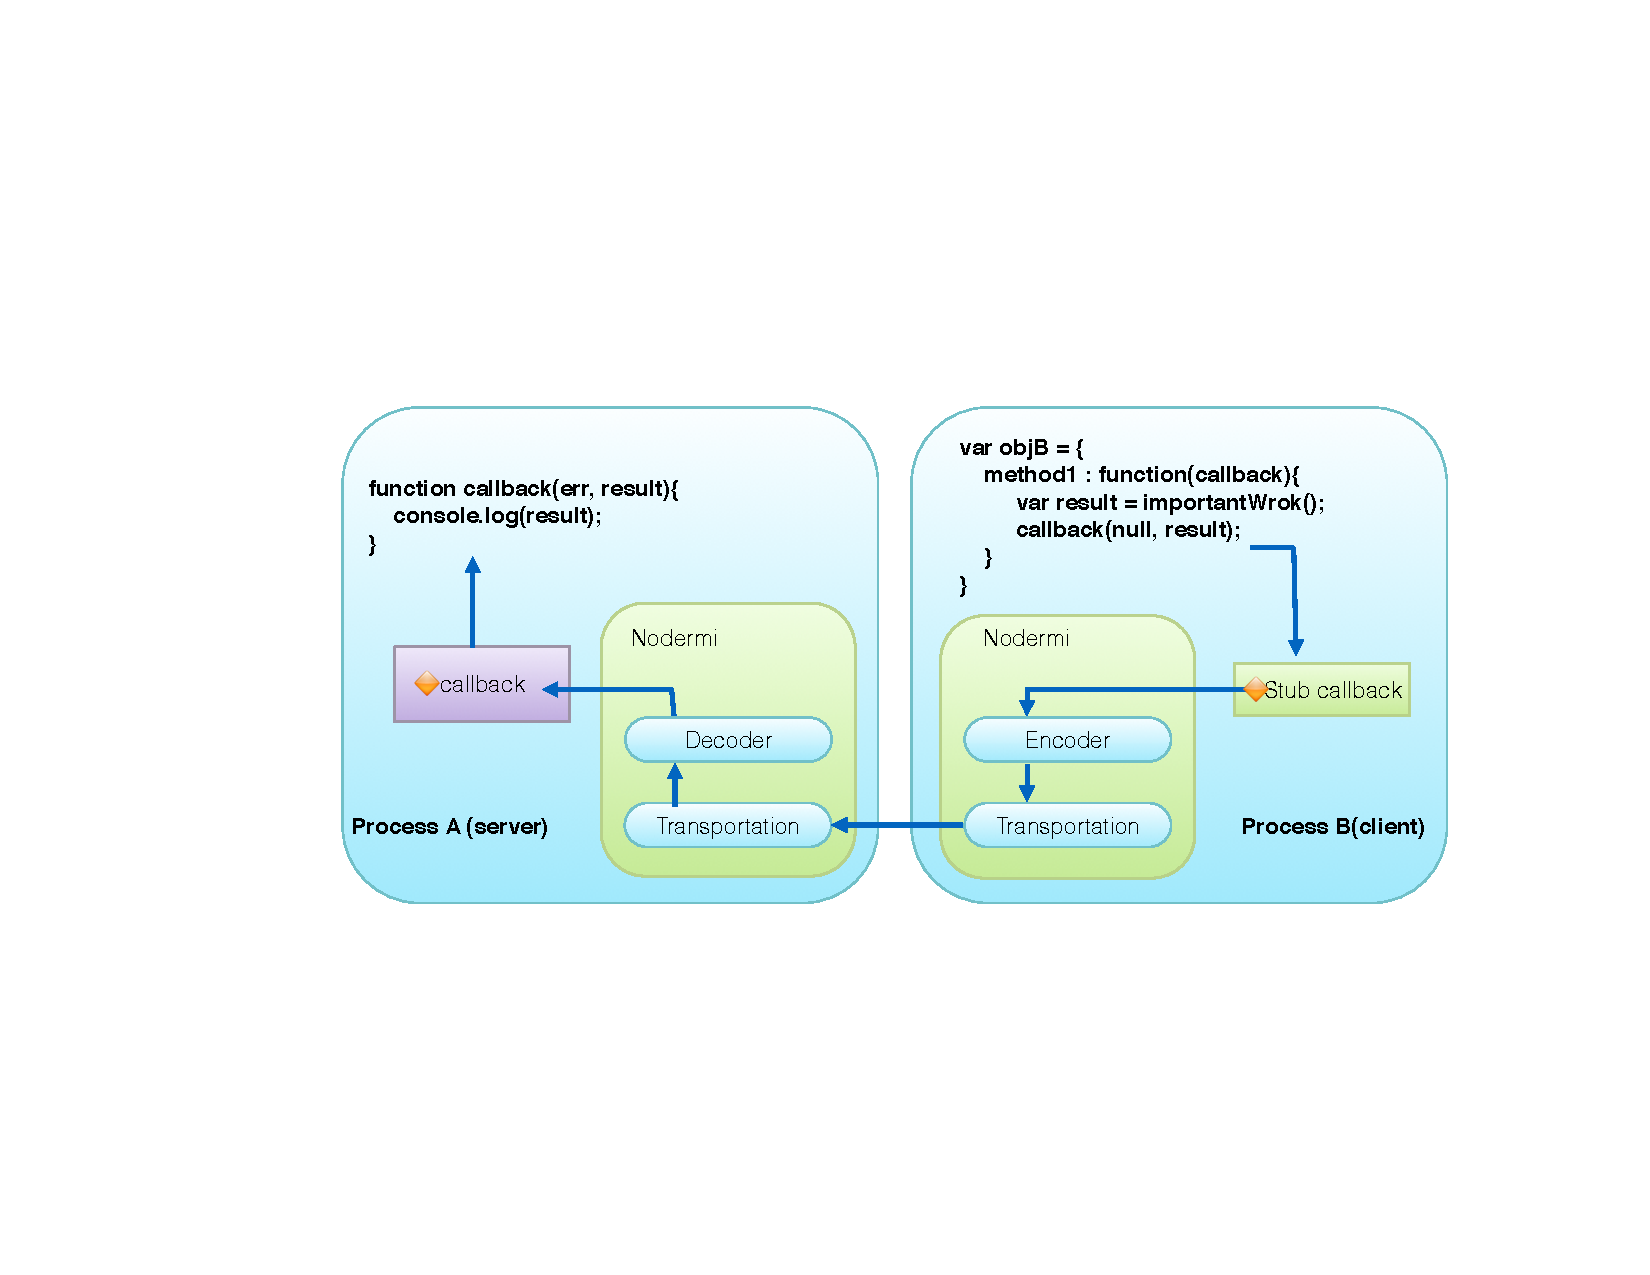
\includegraphics[width=0.8\textwidth]{../figs/nodermi_callback}
    \caption[Remote callback via a stub function]{Process B invoke a callback that itself is a stub}
    \label{fig:nodermicallback}
    \end{figure}
}

\newcommand{\nodermiexamplefig}{
    \begin{figure}[tb]
    \centering
    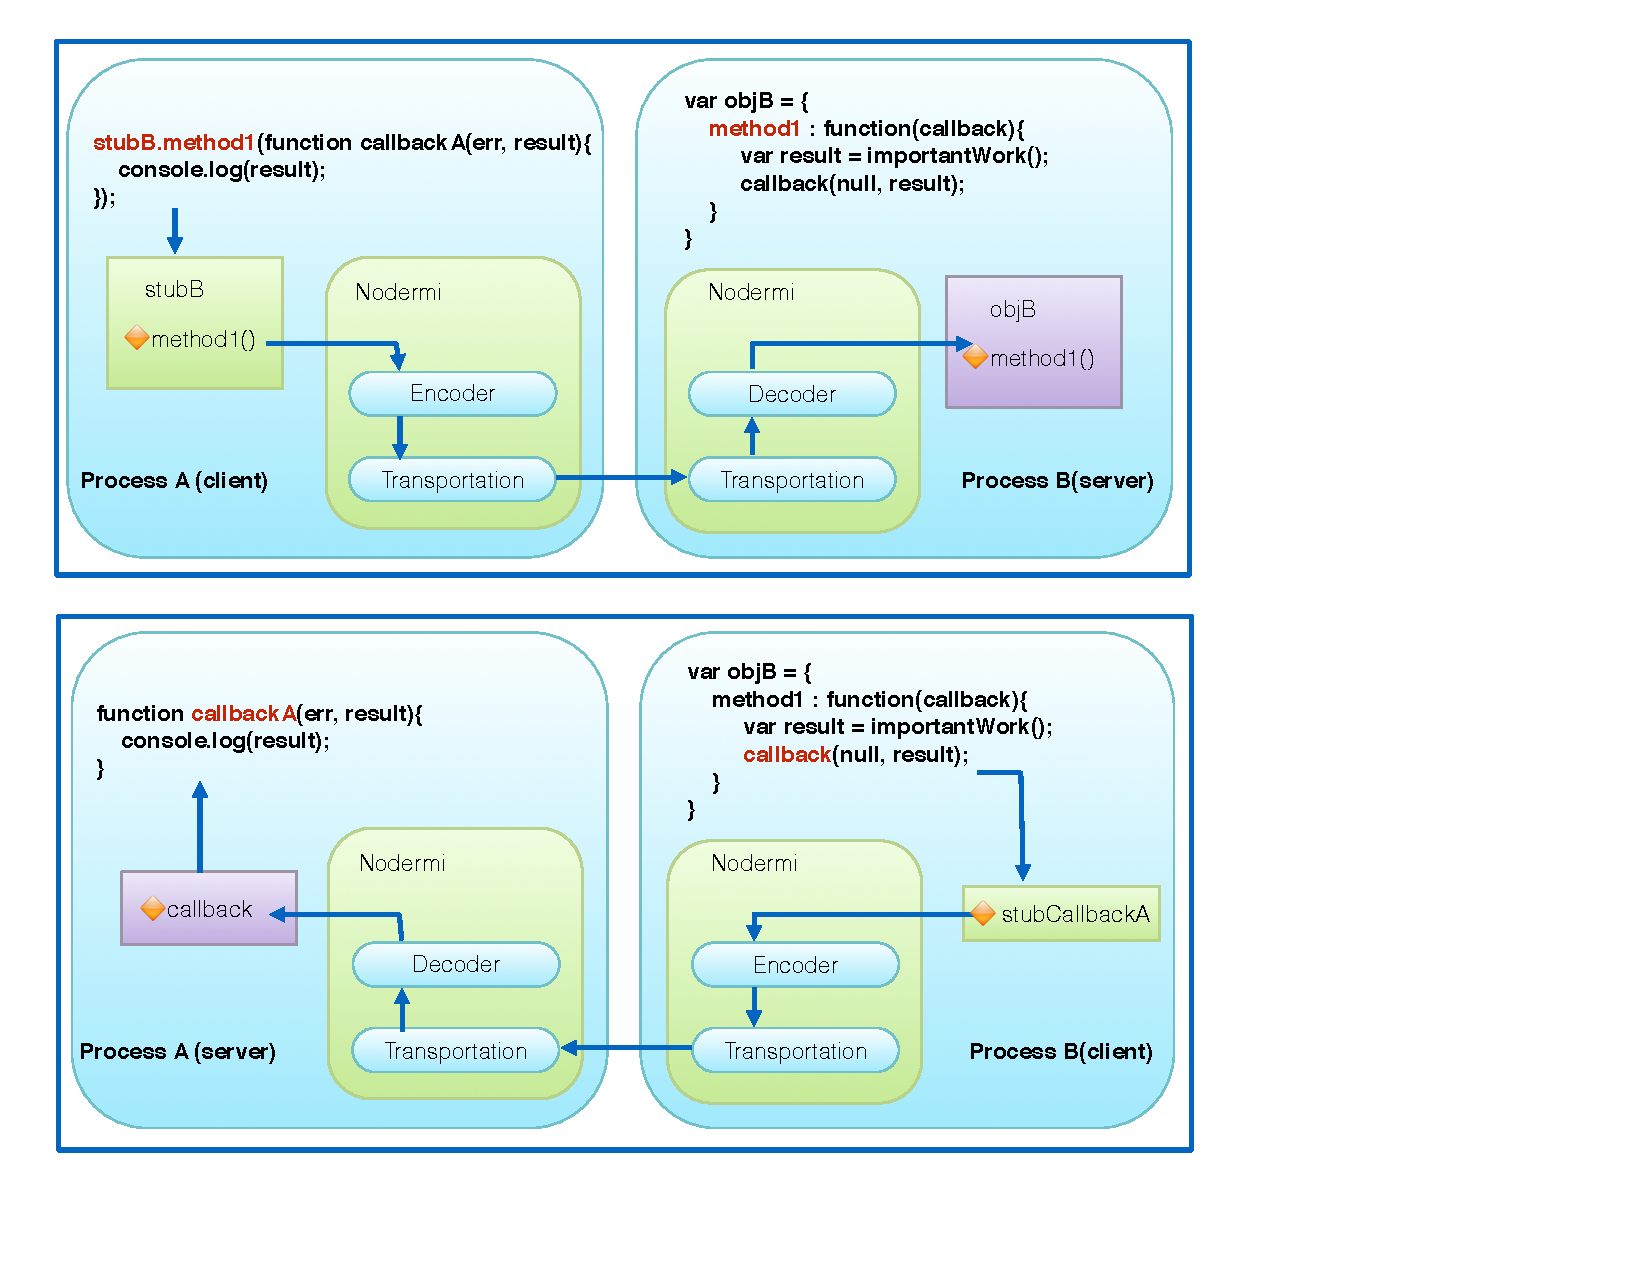
\includegraphics[width=0.8\textwidth]{../figs/nodermi_example}
    \caption{Nodermi remote method invocation example}
    \label{fig:nodermiexample}
    \end{figure}
}

\newcommand{\nodermiobjmapfig}{
    \begin{figure}[tb]
    \centering
    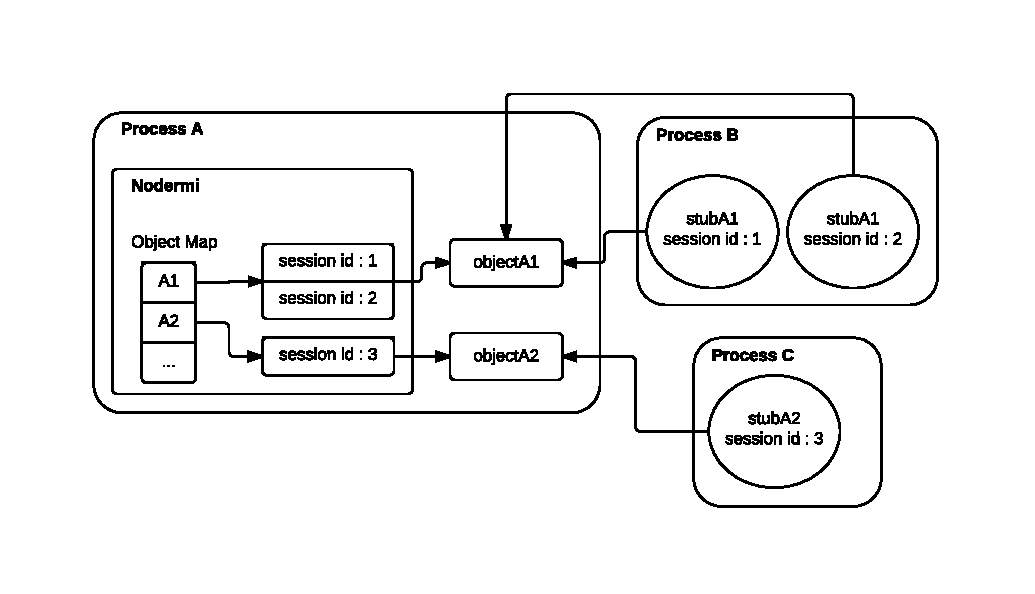
\includegraphics[width=0.8\textwidth]{../figs/nodermi_objectmap}
    \caption[Nodermi memory management]{Nodermi memory management : Nodermi holds 
    strong references to local objects that are remotely referenced in \emph{object map},
    holds weak references to \emph{stub}s in \emph{stub map}.}
    \label{fig:nodermiobjmap}
    \end{figure}
}

%deprecated
\newcommand{\nodermiracefig}{
    \begin{figure}[ht]
    \centering
    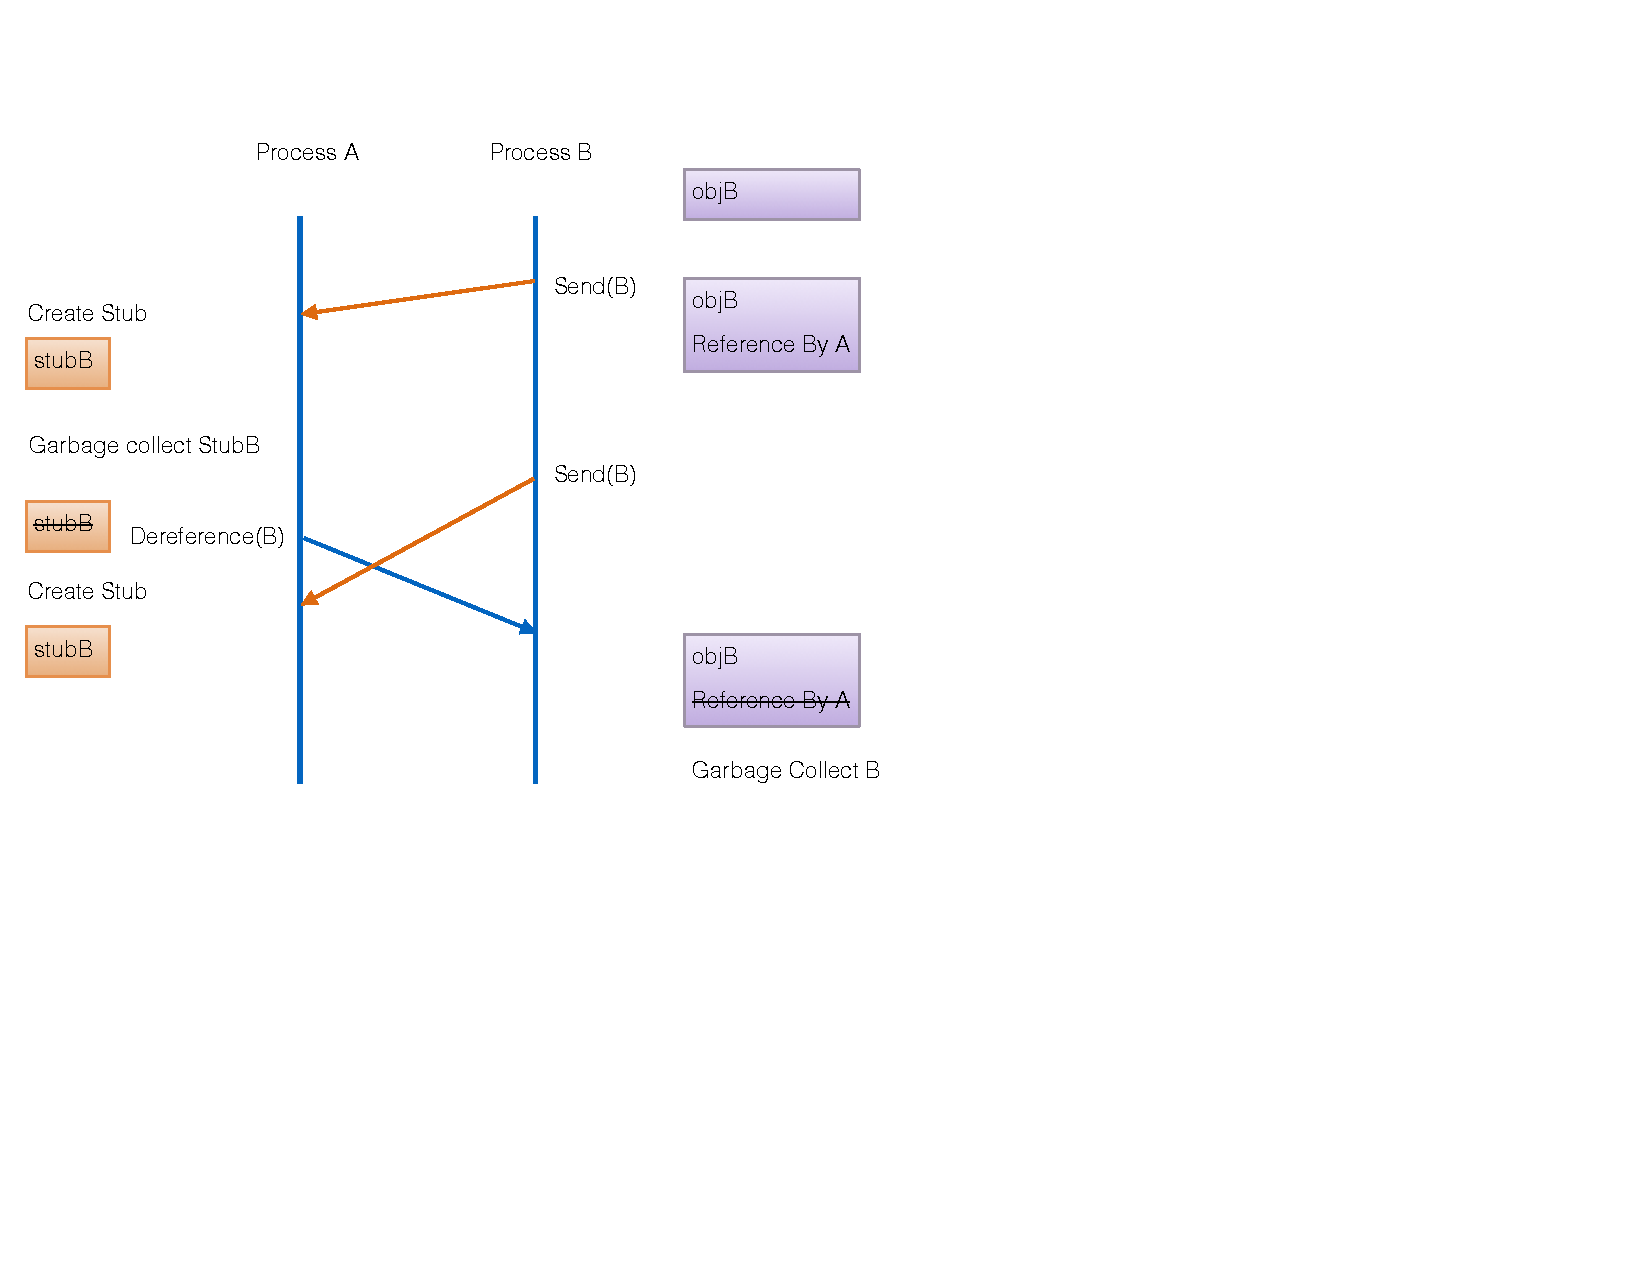
\includegraphics[width=0.8\textwidth]{../figs/nodermi_race}
    \caption[Race condition when dereferencing a remote reference]
    {Race condition when dereferencing a remote reference, \emph{objB} is garbage collected
    when \emph{Process A} still has a stub referencing it.}
    \label{fig:nodermirace}
    \end{figure}
}


\newcommand{\nodermipassbyreffig}{
    \begin{figure}[tb]
    \centering
    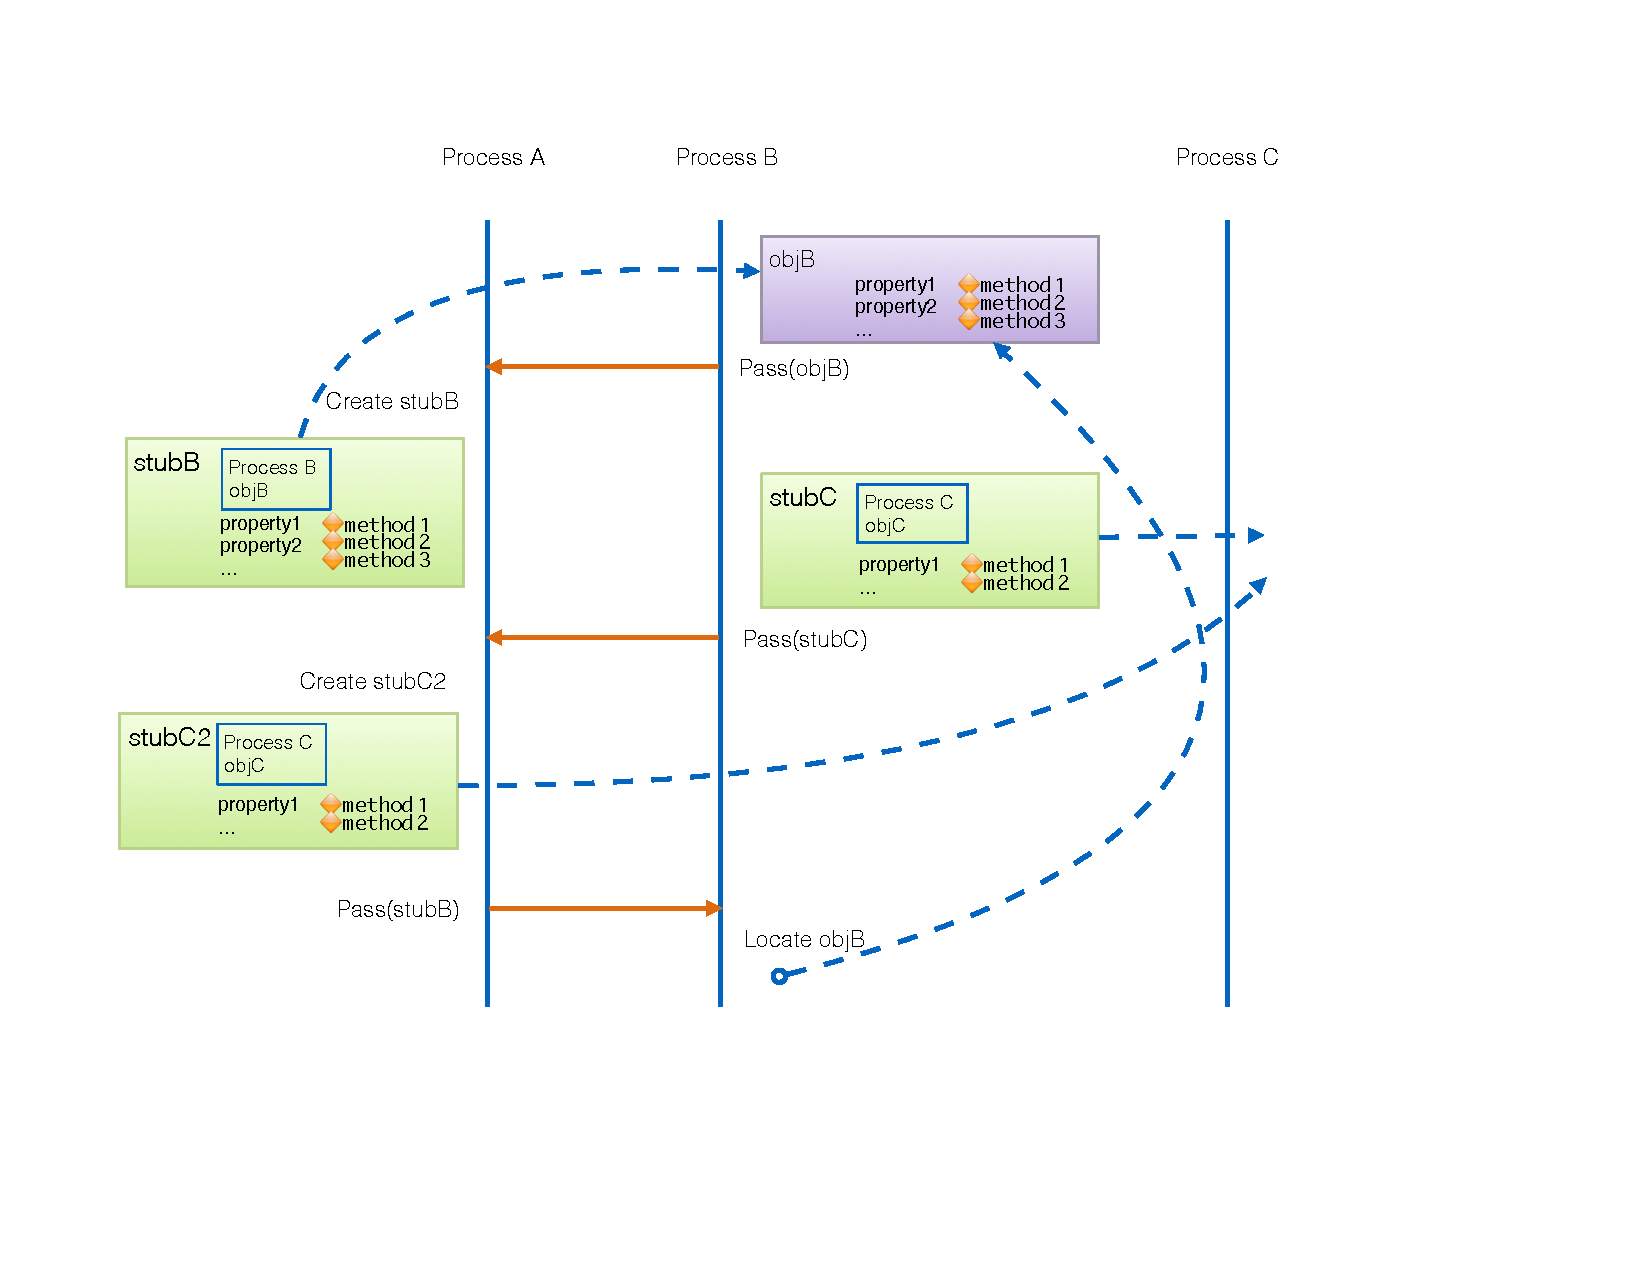
\includegraphics[width=\textwidth]{../figs/nodermi_passbyreference}
    \caption[Nodermi passes arguments by reference]
    {Nodermi passes argument by reference: When passing an argument to a remote
    method call, a remote reference is created for the argument in the server
    process of the remote method. The exception is that 
    when the argument is a stub, nodermi creates
    remote reference for the argument's source object or directly locate
    the source object.}
    \label{fig:nodermipassbyref}
    \end{figure}
}

\newcommand{\nodrmipassbyvalfig}{
    \begin{figure}[tb]
    \centering
    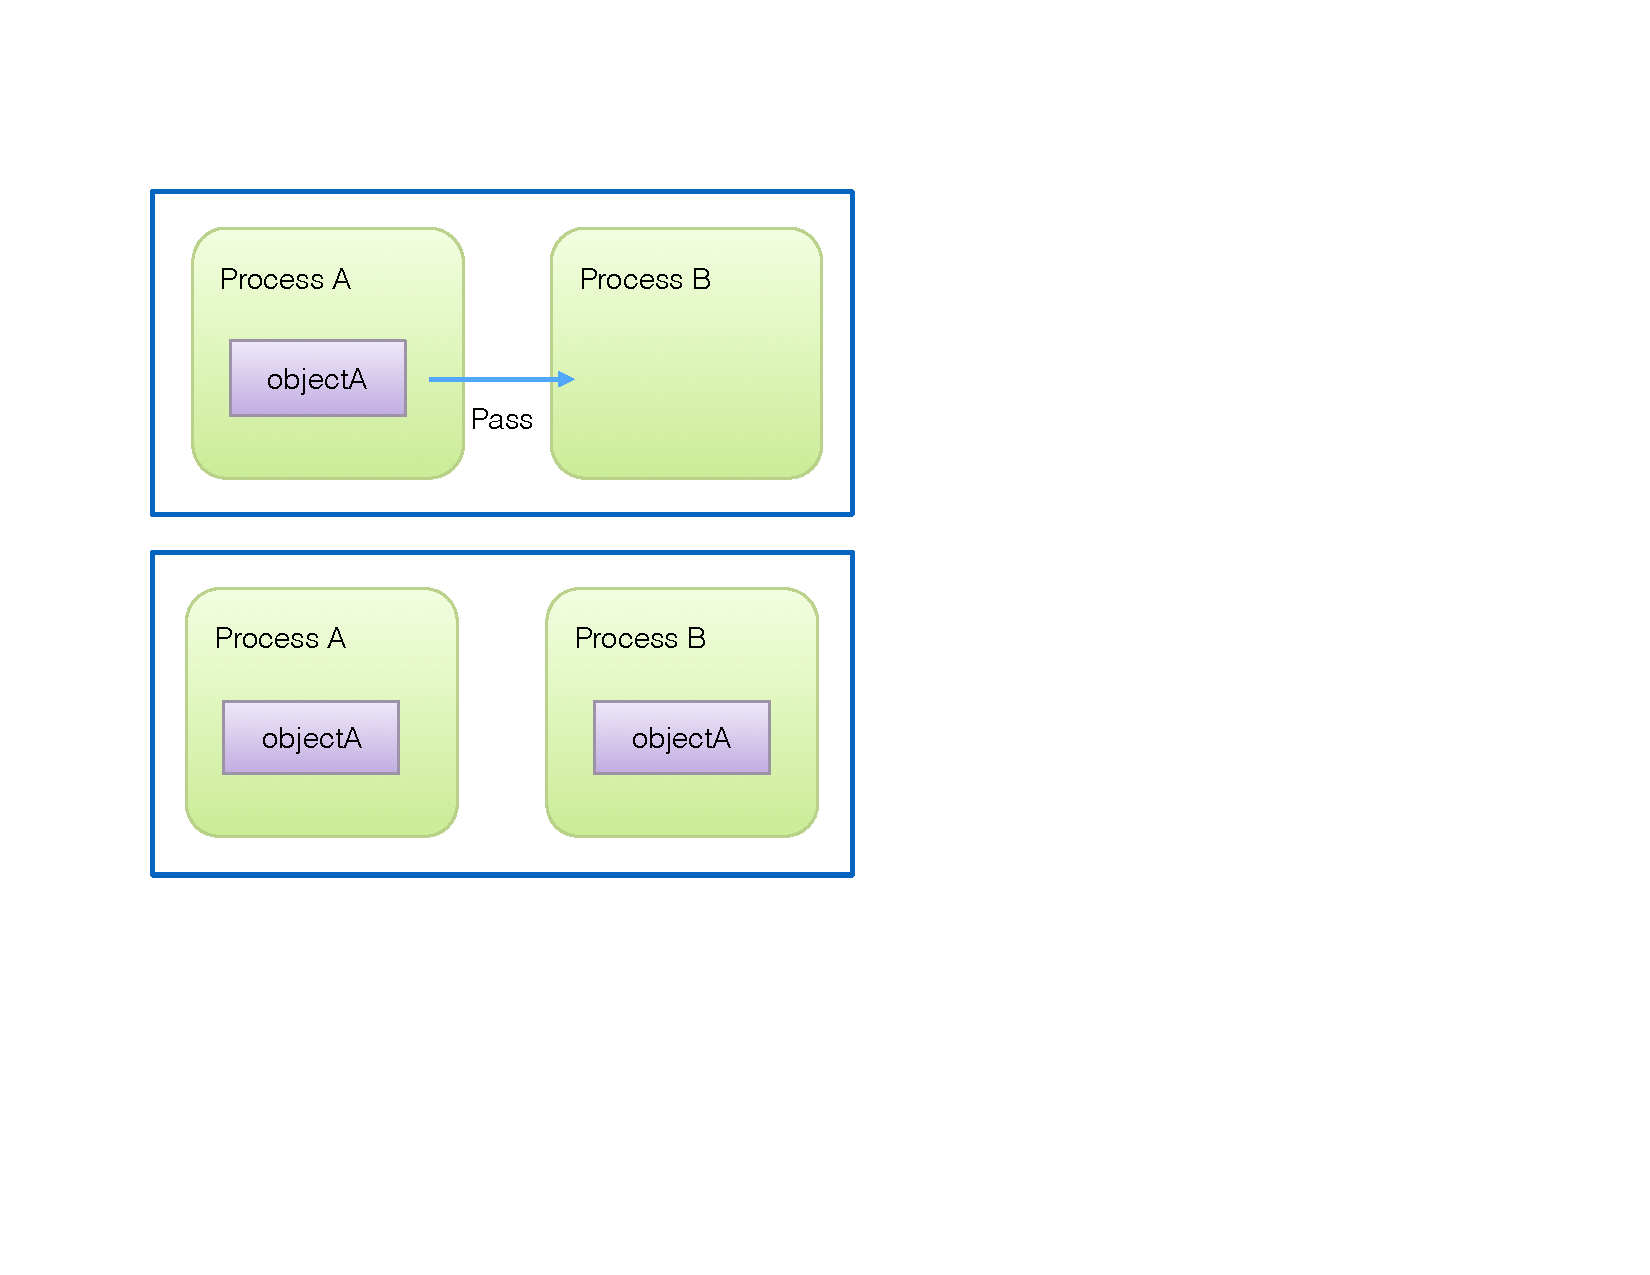
\includegraphics[width=\textwidth]{../figs/nodermi_passbyvalue}
    \caption[Nodermi passes arguments by value]
    {Nodermi passes argument by value: When passing an argument to a remote
    method call and the argument is a simple object with no methods
    , a new copy of the argument is created in the server
    process of the remote method. When the argument is of certain built-in types,
    a new copy is created via constructors, so the new copy has all the methods
    of the original arguments.}
    \label{fig:nodermipassbyval}
    \end{figure}
}

\newcommand{\apiclassfig}{
    \begin{figure}[ht]
    \centering
    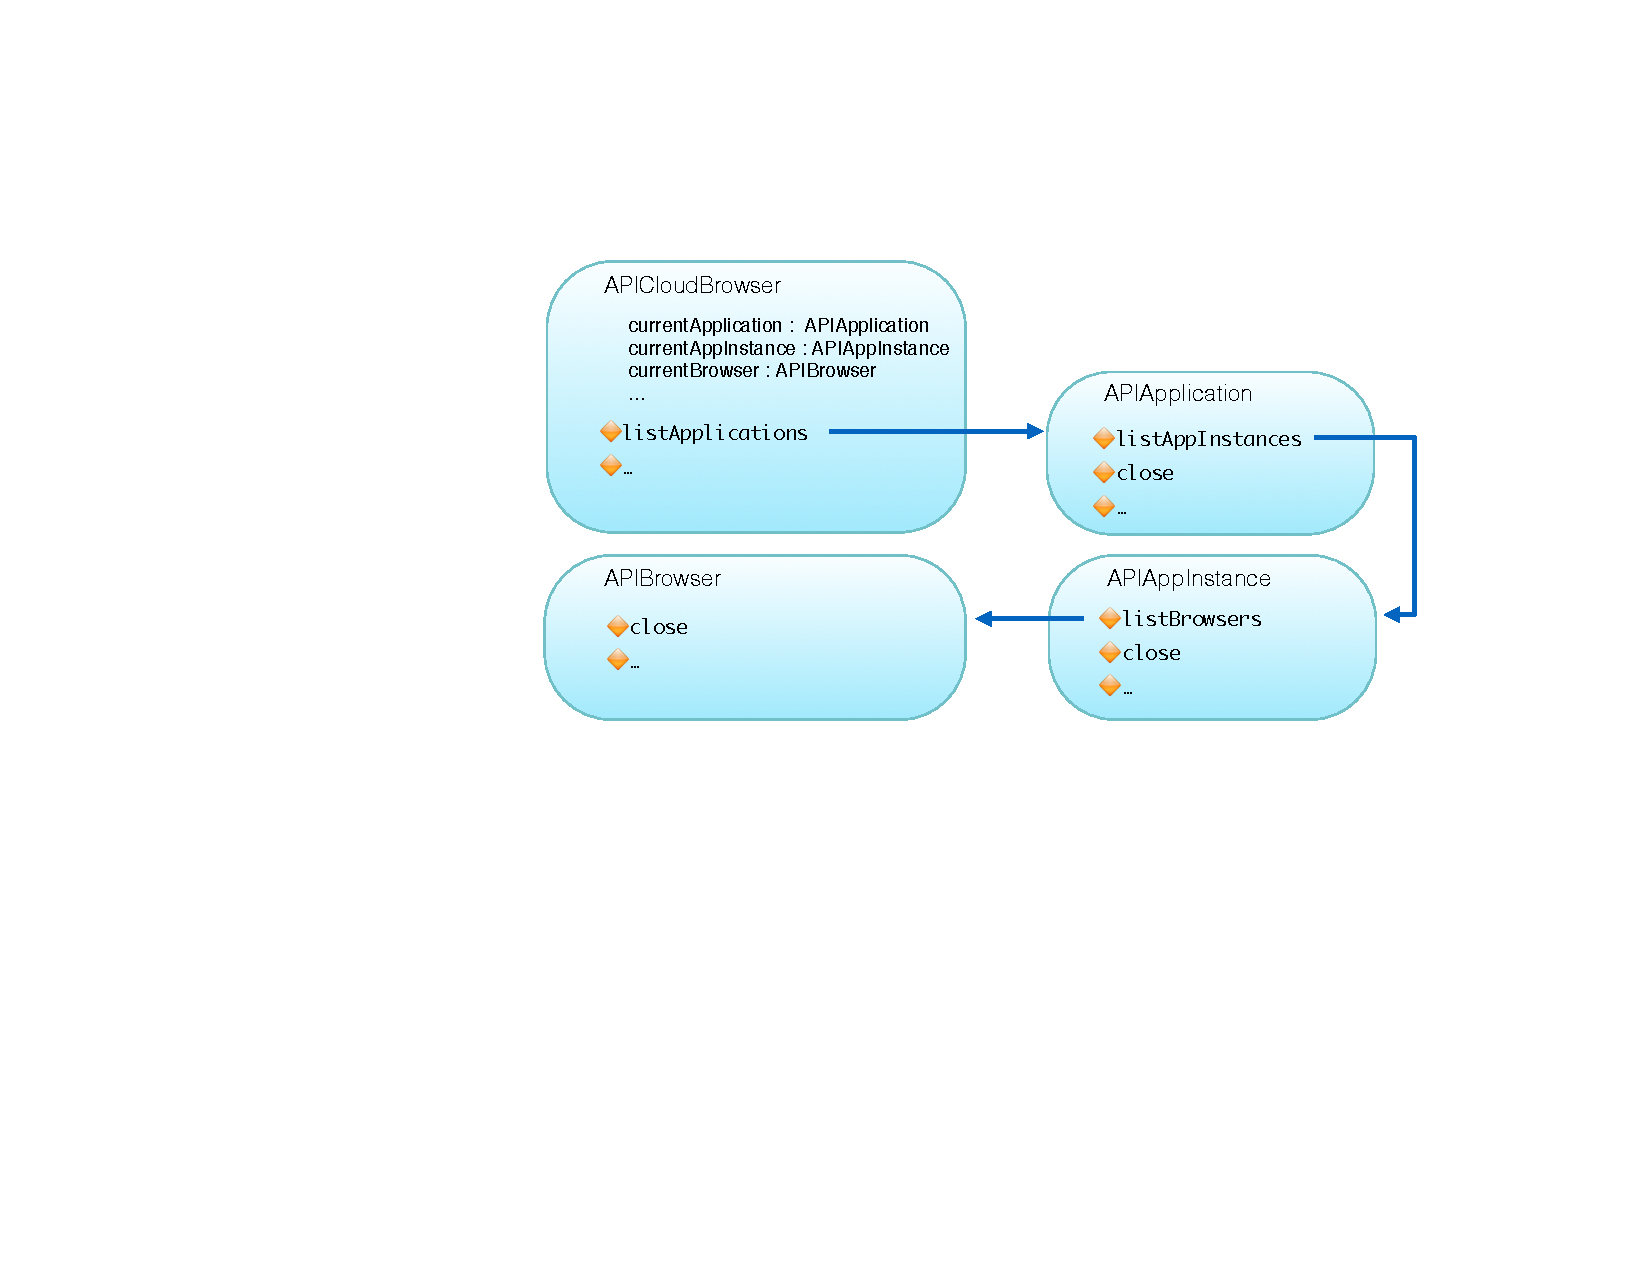
\includegraphics[width=0.8\textwidth]{../figs/api_classes}
    \caption[API class design]{API class design: 
    The arrow points to the method's return value's type.
    For instance,
    The \emph{listApplications} returns
    a list of \emph{APIApplication} objects.
    ``:'' indicates an variable's class, ``currentApplication:APIApplication'' means
     \emph{currentApplication} is a \emph{APIApplication} object.
    }
    \label{fig:apiclass}
    \end{figure}
}


\newcommand{\apireferencefig}{
    \begin{figure}[ht]
    \centering
    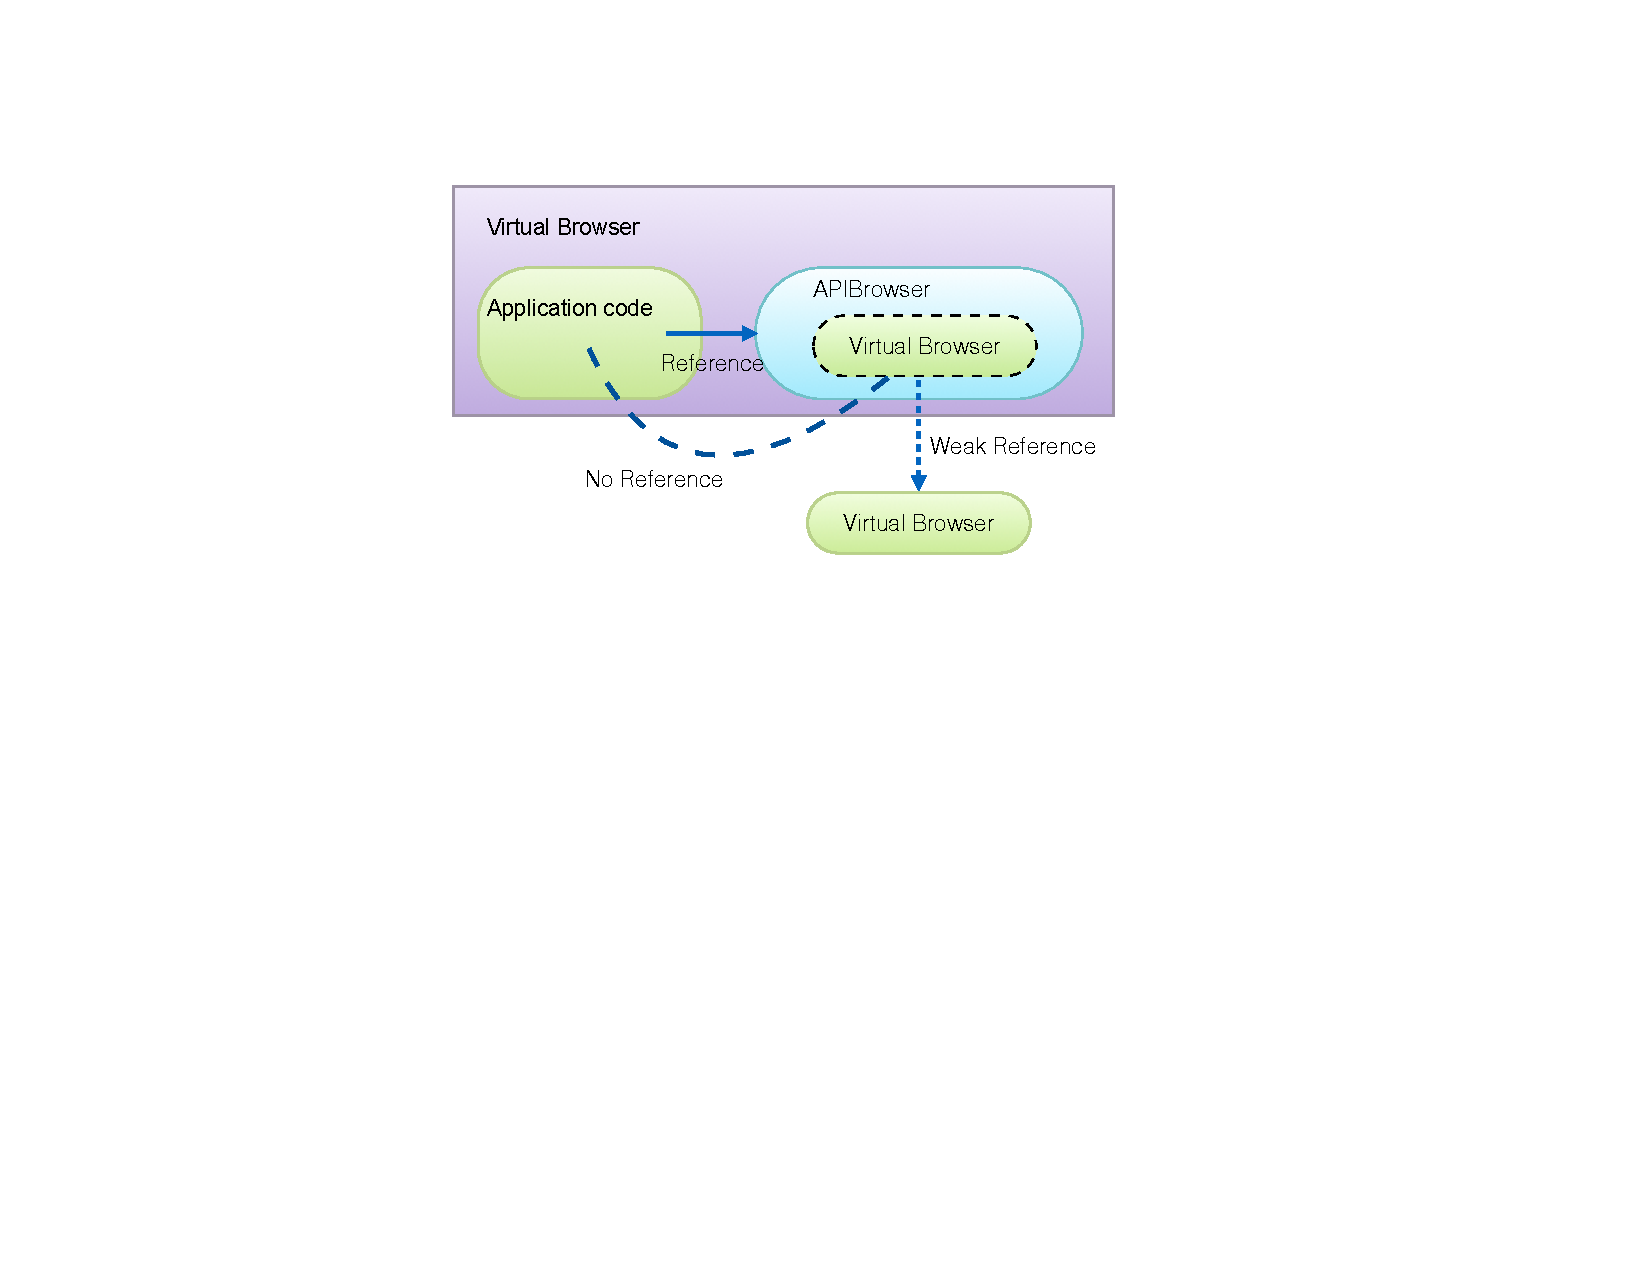
\includegraphics[width=0.6\textwidth]{../figs/api_reference}
    \caption[API object structure]{API object structure : API objects only keep weak reference to internal objects}
    \label{fig:apireference}
    \end{figure}
}